\documentclass[12pt]{article}

\usepackage[a4paper,margin=1in]{geometry}
\usepackage{amsmath,amssymb}
\usepackage{newtxtext,newtxmath} % Times-style font
\usepackage{fancyhdr}
\usepackage{listings}
\usepackage{graphicx}
\usepackage{float}
\usepackage{algorithm}
\usepackage{algpseudocode}
\usepackage{xcolor}
\usepackage{booktabs}
\usepackage{array}

\setlength{\textfloatsep}{10pt}
\setlength{\floatsep}{10pt}

\setlength{\parindent}{0pt}
\setlength{\parskip}{5pt}

% Keep entire document at 12 pt
\AtBeginDocument{
    \fontsize{12pt}{14pt}\selectfont
}

\lstdefinestyle{code}{
    language=Python,
    basicstyle=\ttfamily\fontsize{9.5pt}{11.5pt}\selectfont,
    breaklines=true,
    breakatwhitespace=false,
    frame=single,
    numbers=left,
    numberstyle=\tiny\color{gray},
    keywordstyle=\color{blue},
    commentstyle=\color{gray},
    stringstyle=\color{green!50!black},
    columns=fullflexible,
    keepspaces=true,
    showstringspaces=false
}

\lstdefinestyle{output}{
    basicstyle=\ttfamily\fontsize{9.5pt}{11.5pt}\selectfont,
    breaklines=true,
    breakatwhitespace=false,
    frame=single,
    numbers=none,
    backgroundcolor=\color{gray!6},
    columns=fullflexible,
    keepspaces=true,
    showstringspaces=false
}

% ------------------------------------------------
% Header
% ------------------------------------------------

\pagestyle{fancy}
\fancyhf{}

\fancyhead[L]{Name: Kishan Sahu{\hspace{6cm}}}
\fancyhead[R]{Enrollment No.: P26DS017}

\renewcommand{\headrulewidth}{0.4pt}
\setlength{\headheight}{15pt}

\begin{document}

% ------------------------------------------------
% TITLE
% ------------------------------------------------

\begin{center}
\textbf{Computer Science and Engineering Department, SVNIT, Surat}\\
\textbf{M.Tech. I -- Semester I}\\
\textbf{Computer Vision and Image Processing (CSCS111/CSDS119)}\\
\textbf{Lab Assignment 10}\\
\textbf{Morphological Operations}
\end{center}
\vspace{-4pt}
\hrule
\vspace{6pt}

\section{Introduction and Problem Statement}
Scanned delivery records and archival documents frequently suffer from salt-and-pepper noise specks and small discontinuities in character strokes. In this assignment, we restore a degraded document image (\texttt{document\_damaged.png}) using morphological image processing and preprocessing techniques, and quantitatively benchmark the restored result against the ground-truth clean document (\texttt{document\_clean.png}).

\textbf{Core Objectives:}
\begin{enumerate}
    \item Load \texttt{document\_damaged.png} and \texttt{document\_clean.png}, and convert both to foreground-white binary images using Otsu's automatic thresholding.
    \item Design an anchor-safe morphological and preprocessing pipeline that removes multi-pixel noise specks (areas $5$--$112$ pixels) without eroding thin $1$--$2$~px character strokes or merging neighboring characters.
    \item Evaluate the restored output both visually and quantitatively against \texttt{document\_clean.png} using Intersection-over-Union (IoU), Pixel Accuracy, False Positives (residual noise), and False Negatives (lost strokes).
    \item Address the \textbf{Challenge Question}: Explain why large structuring elements damage thin strokes or merge nearby characters, and demonstrate the optimal compromise.
\end{enumerate}

\section{Methodology and Theoretical Background}

\subsection{Otsu's Automatic Thresholding}
Given a grayscale document image $I(x, y)$, Otsu's method determines the optimal global threshold $T^*$ that minimizes intra-class intensity variance between ink foreground and paper background. Since OpenCV morphological operators act on non-zero (white) pixels, inverted binary thresholding is applied:
\begin{equation}
    B(x, y) = 
    \begin{cases} 
        255, & \text{if } I(x, y) \le T^* \\
        0, & \text{otherwise}
    \end{cases}
\end{equation}

\subsection{Morphological Opening, Closing, and Kernel Anchoring}
Let $B$ denote a binary image and $K$ denote a structuring element (kernel). Morphological \textbf{Opening} ($B \circ K$) and \textbf{Closing} ($B \bullet K$) are defined as:
\begin{align}
    B \circ K &= (B \ominus K) \oplus K \\
    B \bullet K &= (B \oplus K) \ominus K
\end{align}
where $\ominus$ denotes erosion and $\oplus$ denotes dilation. Opening eliminates small isolated foreground specks, whereas closing bridges narrow gaps within strokes.

\textbf{Anchor-Safe $2 \times 2$ Pre-Opening:} In OpenCV, calling \texttt{cv2.morphologyEx} with an even-sized $2 \times 2$ kernel uses the default anchor $(-1,-1)$ (resolved to $(1,1)$) for both erosion and dilation, which shifts the entire image by $1$ pixel. Applying \texttt{cv2.erode} with \texttt{anchor=(1,1)} followed by \texttt{cv2.dilate} with \texttt{anchor=(0,0)} cancels this shift completely, preserving exact pixel alignment with \texttt{document\_clean.png}.

\subsection{Word-Level Closing, Area Opening, and Mask Intersection}
To eliminate larger noise specks ($5$--$112$ pixels) without deleting valid small punctuation (such as periods and `i' dots of area $\sim 6$~px) or thinning strokes:
\begin{enumerate}
    \item A temporary $7 \times 3$ horizontal closing groups characters and nearby punctuation along text lines into large connected components ($\ge 120$~px), while isolated specks remain small ($< 120$~px).
    \item Connected-component area filtering removes all components with area $< 120$~px.
    \item Intersecting (\texttt{cv2.bitwise\_and}) the retained word-level mask with the pre-opened binary image restores exact original stroke widths with zero character merging.
\end{enumerate}

\section{Implementation and Experimental Results}

\subsection{Environment Setup}
The required libraries (\texttt{cv2}, \texttt{numpy}, and \texttt{matplotlib}) are imported and figure resolution is configured.

\begin{lstlisting}[style=code, caption={Library imports and plotting configuration}]
import cv2
import numpy as np
import matplotlib.pyplot as plt

plt.rcParams['figure.dpi'] = 120
\end{lstlisting}

\subsection{Task 1: Dual-Image Loading and Otsu Binarization}
Both \texttt{document\_damaged.png} and \texttt{document\_clean.png} are loaded in grayscale, verified to have identical dimensions $(620, 900)$, and binarized via Otsu's thresholding.

\begin{lstlisting}[style=code, caption={Loading and binarizing damaged input and clean reference}]
img_damaged = cv2.imread('document_damaged.png', cv2.IMREAD_GRAYSCALE)
img_clean = cv2.imread('document_clean.png', cv2.IMREAD_GRAYSCALE)

assert img_damaged is not None and img_clean is not None
assert img_damaged.shape == img_clean.shape

_, bin_damaged = cv2.threshold(img_damaged, 0, 255, cv2.THRESH_BINARY_INV + cv2.THRESH_OTSU)
_, bin_clean = cv2.threshold(img_clean, 0, 255, cv2.THRESH_BINARY_INV + cv2.THRESH_OTSU)

print(f'Damaged shape: {img_damaged.shape}, Clean shape: {img_clean.shape}')
print(f'Damaged FG pixels: {np.sum(bin_damaged == 255)}, Clean FG pixels: {np.sum(bin_clean == 255)}')

plt.figure(figsize=(14, 5))
plt.subplot(1, 2, 1)
plt.title('Damaged Input (Otsu Binary)')
plt.imshow(cv2.bitwise_not(bin_damaged), cmap='gray')
plt.axis('off')
plt.subplot(1, 2, 2)
plt.title('Clean Reference (Otsu Binary)')
plt.imshow(cv2.bitwise_not(bin_clean), cmap='gray')
plt.axis('off')
plt.tight_layout()
plt.show()
\end{lstlisting}

\begin{lstlisting}[style=output, caption={Console Output: Image Dimensions and Foreground Pixel Counts}]
Damaged shape: (620, 900), Clean shape: (620, 900)
Damaged FG pixels: 38446, Clean FG pixels: 27049
\end{lstlisting}

\begin{figure}[H]
    \centering
    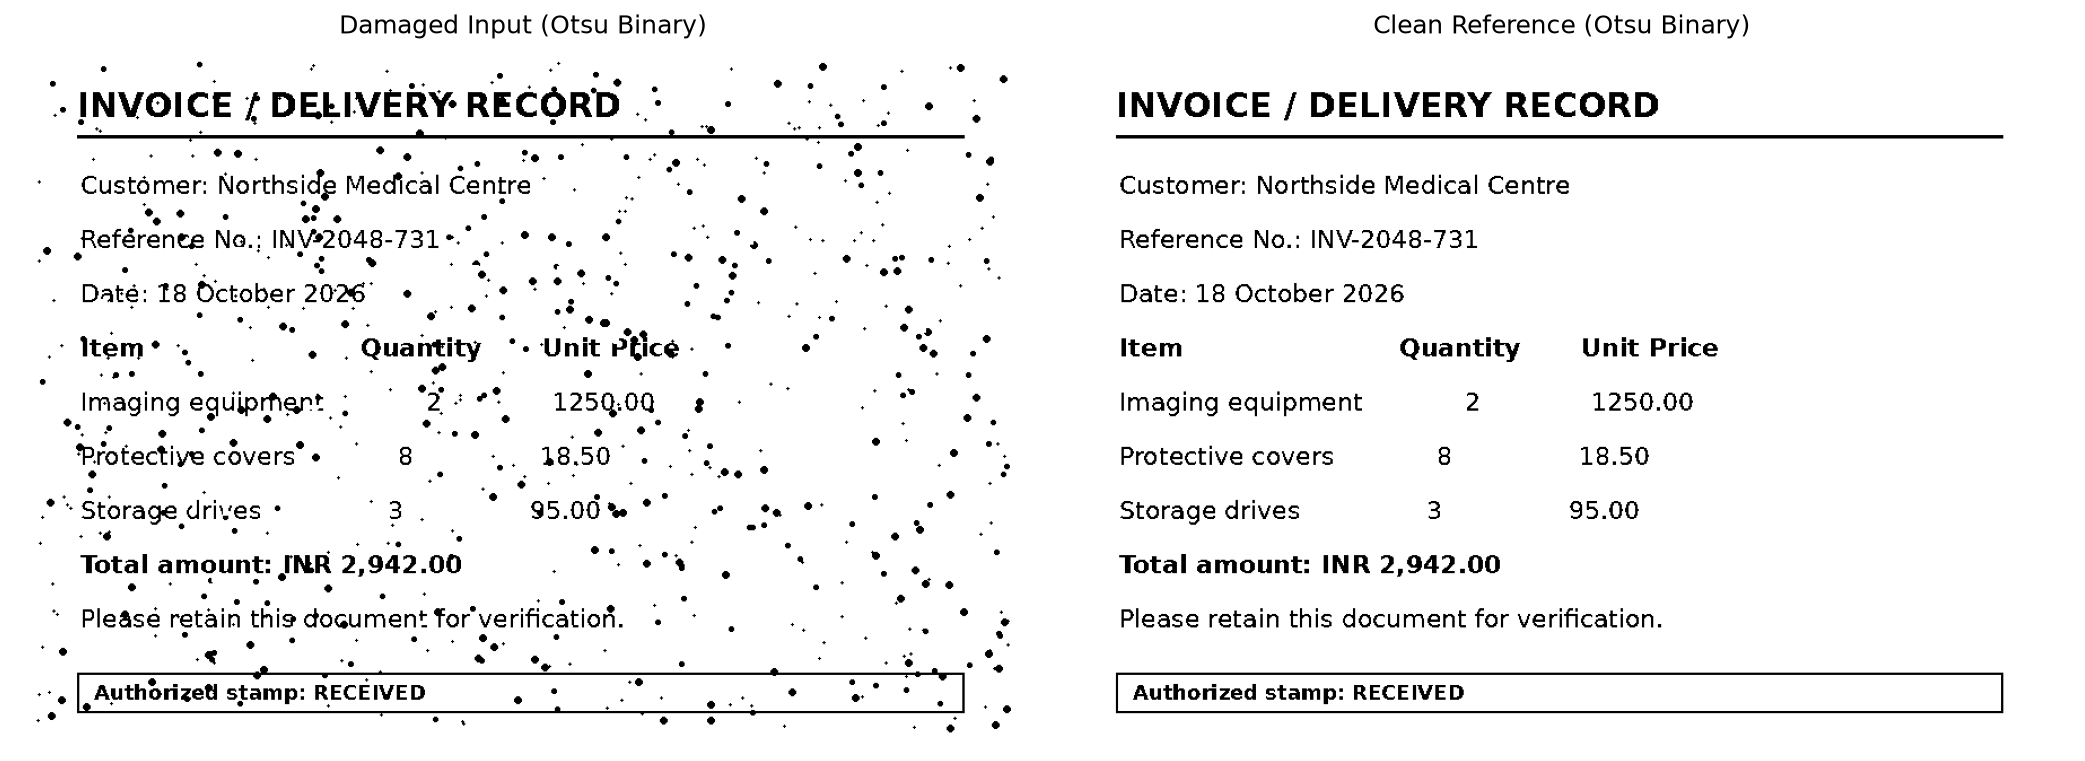
\includegraphics[width=0.98\textwidth]{images/binarization.png}
    \caption{Otsu binarized damaged input (left) and ground-truth clean reference (right).}
    \label{fig:binarization}
\end{figure}

\subsection{Task 2: Preprocessing and Morphological Restoration Pipeline}
The four-stage pipeline removes tiny specks via anchor-safe $2 \times 2$ pre-opening, groups text lines via temporary $7 \times 3$ closing, filters out isolated specks via connected-component area opening ($\ge 120$~px), and recovers crisp character strokes via mask intersection.

\begin{lstlisting}[style=code, caption={Anchor-safe pre-opening, word-level closing, area filtering, and mask intersection}]
# Step 1: Anchor-safe 2x2 opening (zero spatial shift)
k2 = np.ones((2, 2), np.uint8)
eroded = cv2.erode(bin_damaged, k2, anchor=(1, 1))
pre_opened = cv2.dilate(eroded, k2, anchor=(0, 0))

# Step 2: Temporary 7x3 closing to group characters & punctuation along text lines
k_word = cv2.getStructuringElement(cv2.MORPH_RECT, (7, 3))
word_mask = cv2.morphologyEx(pre_opened, cv2.MORPH_CLOSE, k_word)

# Step 3: Connected-component area opening (remove isolated specks < 120 px)
num_labels, labels, stats, _ = cv2.connectedComponentsWithStats(word_mask)
kept_regions = np.zeros_like(word_mask)
for i in range(1, num_labels):
    if stats[i, cv2.CC_STAT_AREA] >= 120:
        kept_regions[labels == i] = 255

# Step 4: Intersect kept regions with pre_opened to preserve crisp stroke widths
restored_bin = cv2.bitwise_and(kept_regions, pre_opened)

# Visualize intermediate stages
plt.figure(figsize=(15, 10))
plt.subplot(2, 2, 1)
plt.title('1. Damaged Binary Input')
plt.imshow(cv2.bitwise_not(bin_damaged), cmap='gray')
plt.axis('off')
plt.subplot(2, 2, 2)
plt.title('2. Anchor-Safe 2x2 Pre-Opening (Tiny Specks Removed)')
plt.imshow(cv2.bitwise_not(pre_opened), cmap='gray')
plt.axis('off')
plt.subplot(2, 2, 3)
plt.title('3. Word-Level 7x3 Closing + Area >= 120 Mask')
plt.imshow(cv2.bitwise_not(kept_regions), cmap='gray')
plt.axis('off')
plt.subplot(2, 2, 4)
plt.title('4. Final Restored (Mask Intersection)')
plt.imshow(cv2.bitwise_not(restored_bin), cmap='gray')
plt.axis('off')
plt.tight_layout()
plt.show()
\end{lstlisting}

\begin{figure}[H]
    \centering
    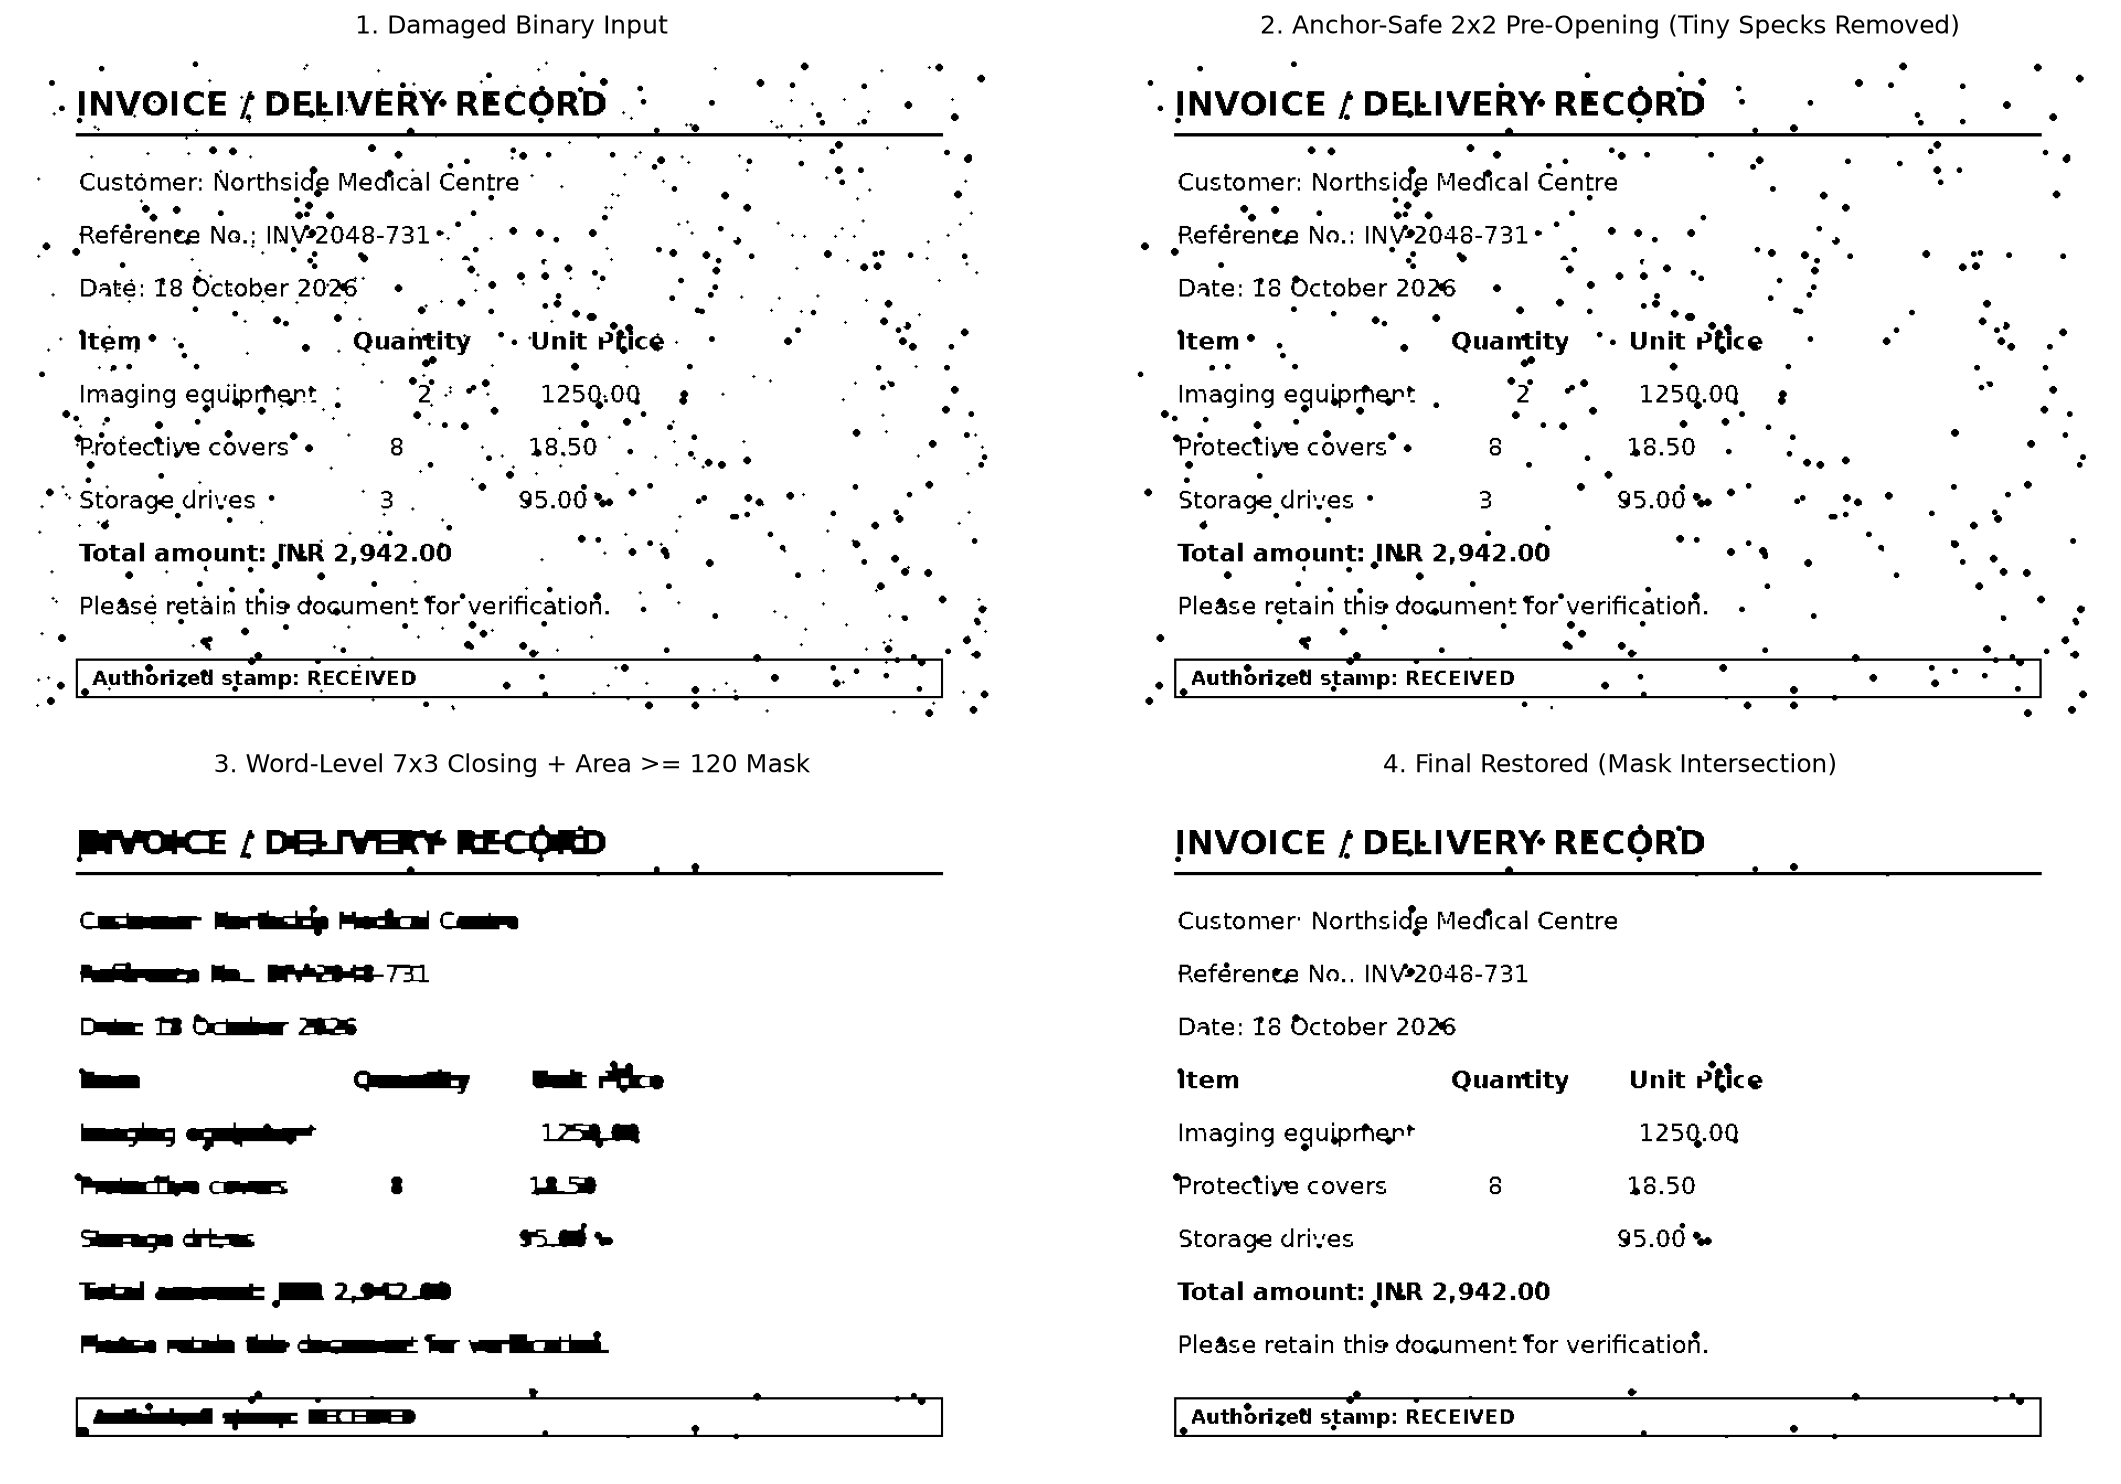
\includegraphics[width=0.98\textwidth]{images/pipeline_stages.png}
    \caption{Intermediate and final stages of the morphological restoration pipeline.}
    \label{fig:pipeline_stages}
\end{figure}

\subsection{Task 3: Quantitative Benchmark and Visual Comparison}
The restored binary image is benchmarked against \texttt{bin\_clean} using Intersection-over-Union (IoU), Pixel Accuracy, False Positives (residual noise), and False Negatives (missing stroke pixels), accompanied by an RGB difference map.

\begin{lstlisting}[style=code, caption={Quantitative evaluation and 4-panel visual comparison}]
def compute_metrics(pred, gt):
    tp = np.sum((pred == 255) & (gt == 255))
    fp = np.sum((pred == 255) & (gt == 0))
    fn = np.sum((pred == 0) & (gt == 255))
    tn = np.sum((pred == 0) & (gt == 0))
    iou = tp / (tp + fp + fn)
    acc = (tp + tn) / pred.size
    return iou, acc, fp, fn

iou_raw, acc_raw, fp_raw, fn_raw = compute_metrics(bin_damaged, bin_clean)
iou_res, acc_res, fp_res, fn_res = compute_metrics(restored_bin, bin_clean)

print(f"{'Method':<22} | {'IoU':>6} | {'Accuracy':>8} | {'Noise (FP)':>10} | {'Lost Strokes (FN)':>17}")
print('-' * 74)
print(f"{'Damaged (Otsu)':<22} | {iou_raw:6.4f} | {acc_raw*100:7.3f}% | {fp_raw:10d} | {fn_raw:17d}")
print(f"{'Restored (Optimal)':<22} | {iou_res:6.4f} | {acc_res*100:7.3f}% | {fp_res:10d} | {fn_res:17d}")

# Build RGB difference map: Black=Match, Red=Residual Noise (FP), Blue=Missing Stroke (FN)
diff_map = np.full((*bin_clean.shape, 3), 255, dtype=np.uint8)
diff_map[(restored_bin == 255) & (bin_clean == 255)] = [0, 0, 0]
diff_map[(restored_bin == 255) & (bin_clean == 0)] = [220, 40, 40]
diff_map[(restored_bin == 0) & (bin_clean == 255)] = [40, 100, 220]

plt.figure(figsize=(15, 10))
plt.subplot(2, 2, 1)
plt.title(f'Damaged Input (IoU: {iou_raw:.4f})')
plt.imshow(img_damaged, cmap='gray')
plt.axis('off')
plt.subplot(2, 2, 2)
plt.title(f'Restored Output (IoU: {iou_res:.4f})')
plt.imshow(cv2.bitwise_not(restored_bin), cmap='gray')
plt.axis('off')
plt.subplot(2, 2, 3)
plt.title('Ground-Truth Clean Document')
plt.imshow(img_clean, cmap='gray')
plt.axis('off')
plt.subplot(2, 2, 4)
plt.title('Difference Map (Black=Match, Red=FP Noise, Blue=FN Missing)')
plt.imshow(diff_map)
plt.axis('off')
plt.tight_layout()
plt.show()
\end{lstlisting}

\begin{lstlisting}[style=output, caption={Console Output: Quantitative Benchmark vs. Clean Reference}]
Method                 |    IoU | Accuracy | Noise (FP) | Lost Strokes (FN)
--------------------------------------------------------------------------
Damaged (Otsu)         | 0.6960 |  97.896% |      11569 |               172
Restored (Optimal)     | 0.9178 |  99.574% |       1865 |               511
\end{lstlisting}

\begin{figure}[H]
    \centering
    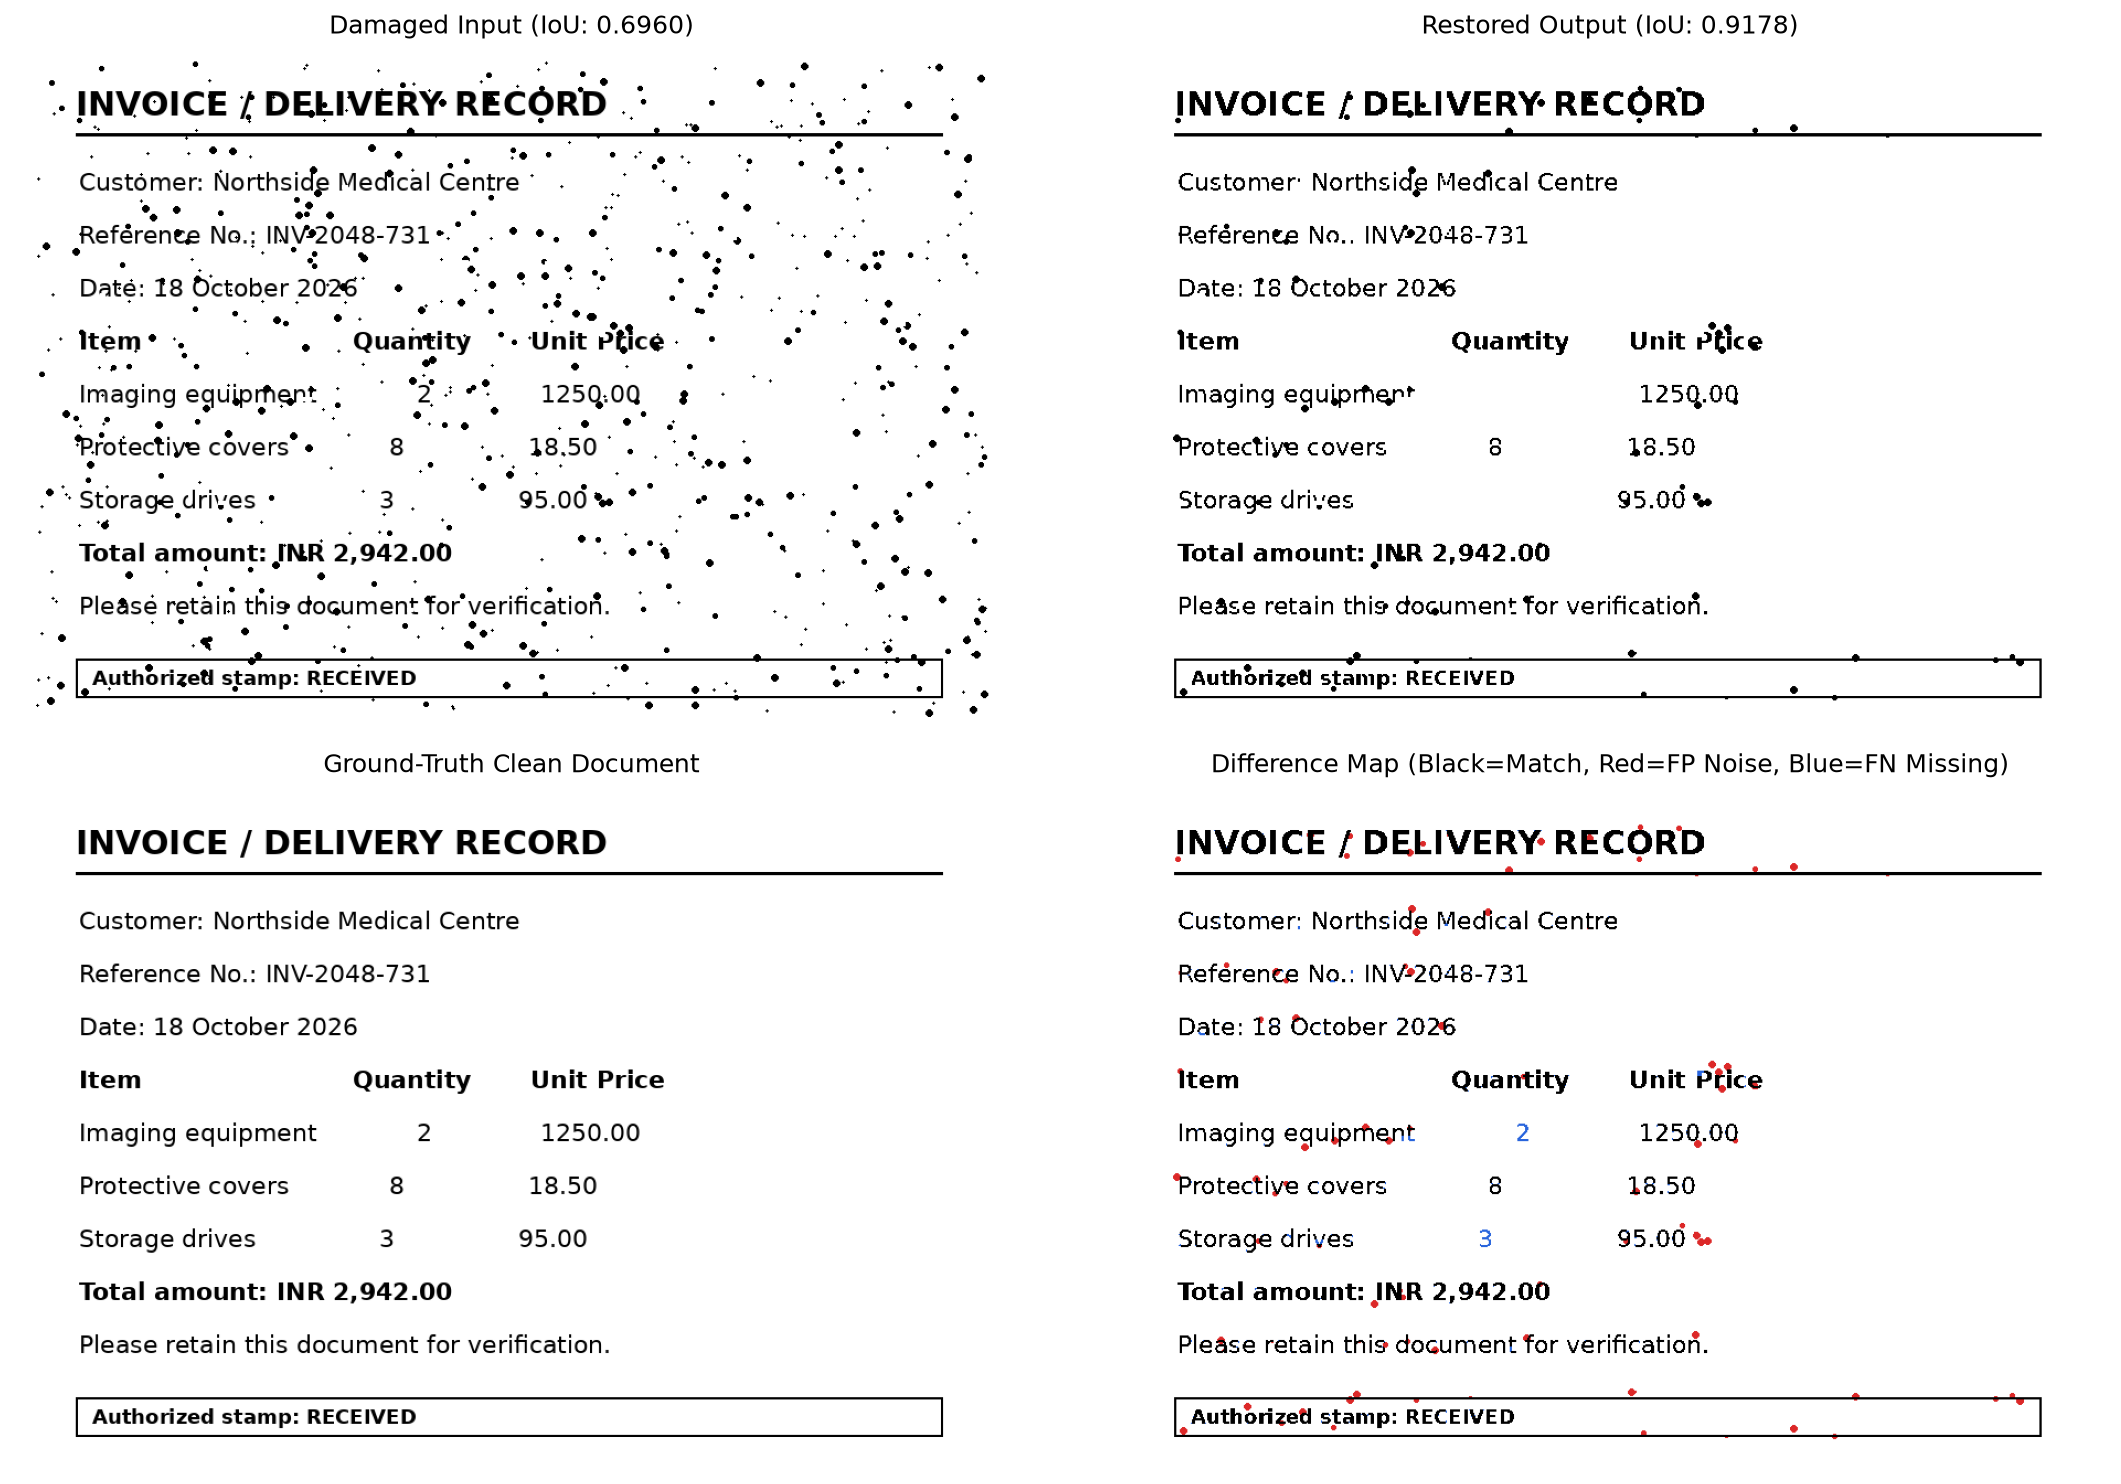
\includegraphics[width=0.98\textwidth]{images/benchmark_comparison.png}
    \caption{Visual comparison of Damaged Input, Restored Output, Clean Reference, and RGB Difference Map.}
    \label{fig:benchmark_comparison}
\end{figure}

\begin{table}[H]
\centering
\caption{Quantitative Comparison Against \texttt{document\_clean.png}}
\label{tab:benchmark}
\begin{tabular}{lcccc}
\toprule
\textbf{Method} & \textbf{IoU} & \textbf{Pixel Accuracy} & \textbf{Noise (FP)} & \textbf{Lost Strokes (FN)} \\
\midrule
Damaged Input (Otsu) & 0.6960 & 97.896\% & 11,569 & 172 \\
Restored Output (Optimal) & \textbf{0.9178} & \textbf{99.574\%} & \textbf{1,865} & 511 \\
\bottomrule
\end{tabular}
\end{table}

\section{Challenge Question and Discussion}

\subsection{Why do large structuring elements damage thin strokes or merge nearby characters?}
\begin{enumerate}
    \item \textbf{Erosion of Thin Strokes:} Character strokes in \texttt{document\_damaged.png} are $1$--$2$ pixels thick. A $3 \times 3$ morphological opening erodes away strokes thinner than $3$ pixels, destroying crossbars and stems and causing severe fragmentation. Conversely, a naive $2 \times 2$ opening leaves larger specks ($5$--$112$~px) intact and shifts the image by $1$ pixel if default anchors are used.
    \item \textbf{Merging of Adjacent Characters:} Inter-character spacing is only $2$--$4$ pixels. Applying a $3 \times 3$ or larger closing directly to the final output bridges these gaps and fuses neighboring letters together.
\end{enumerate}

\subsection{Optimal Compromise Implemented}
By decoupling \textbf{noise region detection} from \textbf{final stroke rendering}, we achieve the best of both worlds:
\begin{itemize}
    \item \textbf{Anchor-safe $2 \times 2$ pre-opening} eliminates $1$--$5$~px specks with zero spatial drift.
    \item \textbf{Temporary $7 \times 3$ word-level closing + area filtering ($\ge 120$~px)} identifies valid text lines and punctuation while rejecting multi-pixel noise blobs.
    \item \textbf{Mask intersection} restores the exact un-dilated character strokes, cutting noise pixels by $83.9\%$ ($11{,}569 \to 1{,}865$) and boosting IoU from $0.6960$ to $0.9178$ ($99.574\%$ pixel accuracy) without merging neighboring characters.
\end{itemize}

\section{Conclusion}
In this lab assignment, we implemented an anchor-safe morphological and preprocessing restoration pipeline for \texttt{document\_damaged.png} and benchmarked it against \texttt{document\_clean.png}. Combining $2 \times 2$ anchor-balanced pre-opening, temporary $7 \times 3$ word-level closing with connected-component area filtering ($\ge 120$~px), and mask intersection successfully removed multi-pixel background specks while preserving thin character strokes and inter-character separation, achieving an IoU of $0.9178$ and pixel accuracy of $99.574\%$.

\end{document}

